\begin{surferPage}[D5-- Singularity]{$D_5^{--}$ Singularity}
Compared to the $D_5^{+-}$ singularity the $D_5^{--}$ singularity might look a bit boring at first sight (the red surface at the left).
    \vspace*{-0.4em}
    \begin{center}
      $x^2y-y^4-z^2=0.$
    \end{center}
    \vspace*{-0.4em}

But even over the real numbers their geometries are closely related to each other (only the sign in front of the $y^4$ differs).
Indeed, close to the singular point the shape of the $D_5^{--}$ fits perfectly into the shape of the $D_5^{+-}$ (in blue at the right).

    \begin{center}
      \begin{tabular}{@{}c@{\quad}c@{\quad}c@{}}
        \begin{tabular}{@{}c@{}}
          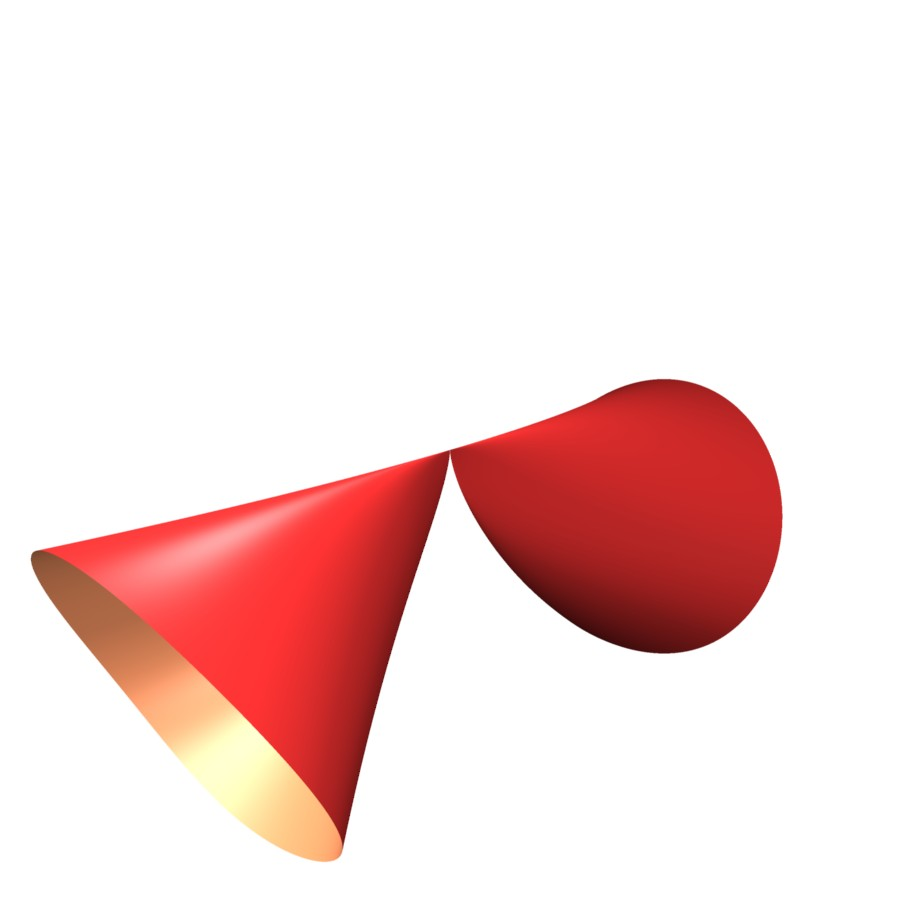
\includegraphics[width=1.1cm]{../../common/images/D5mm_01}
        \end{tabular}
        &
        \begin{tabular}{@{}c@{}}
          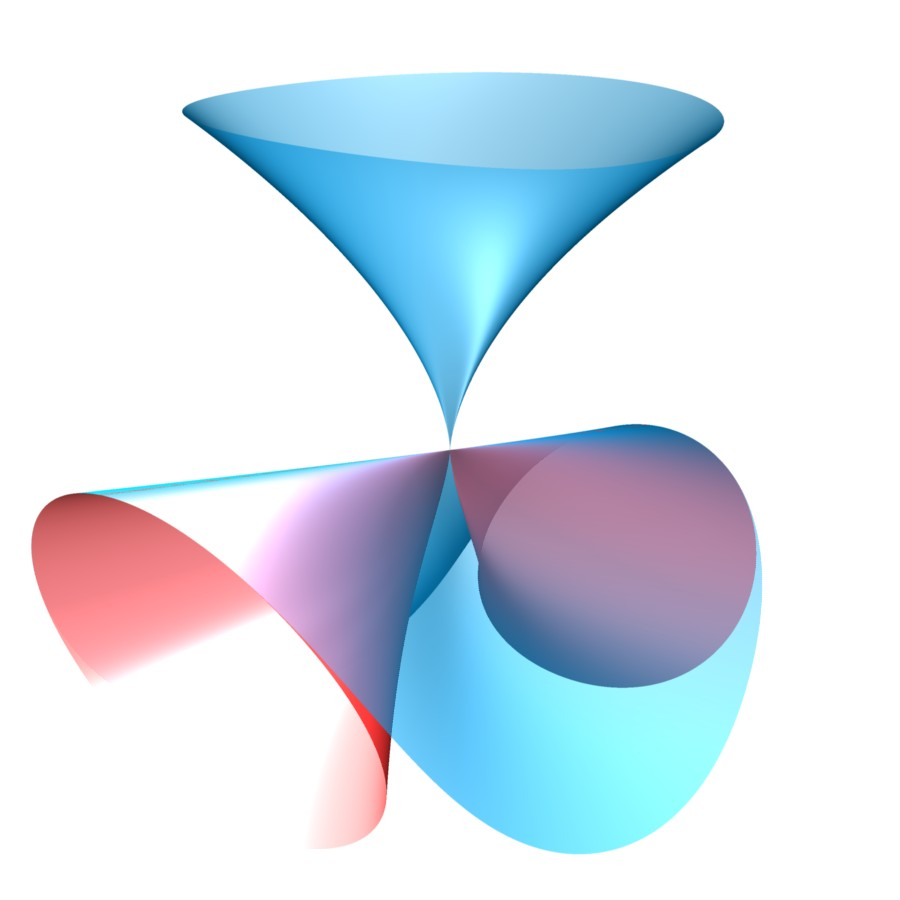
\includegraphics[width=1.1cm]{../../common/images/D5pm_D5mm}
        \end{tabular}
        &
        \begin{tabular}{@{}c@{}}
          
\includegraphics[width=1.1cm]{../../common/images/D5pm_blue}
        \end{tabular}
      \end{tabular}
    \end{center}
    \vspace*{-0.4em}

Interestingly enough, also for the $D_5^{--}$ singularity there exist deformation yielding the same
real types of lower singularities that we were able to get in the $D_5^{+-}$ case.
So, also here it is possible to experience how the $D_5$ develops from the $D_4$; but now by shrinking
the upper part until it is reduced to a point.

    \begin{center}
      \begin{tabular}{@{}c@{\quad}c@{\quad}c@{}}
        \begin{tabular}{@{}c@{}}
          
\includegraphics[width=1.1cm]{../../common/images/D5mm_03}
        \end{tabular}
        &
        \begin{tabular}{@{}c@{}}
          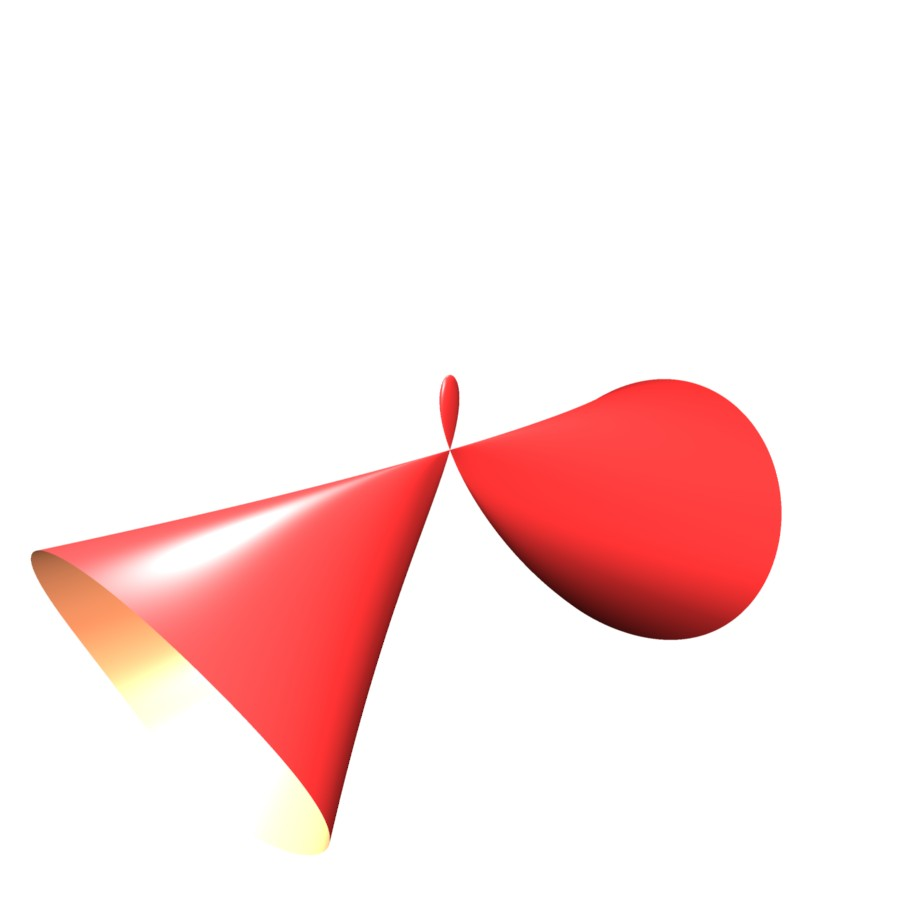
\includegraphics[width=1.1cm]{../../common/images/D5mm_02}
        \end{tabular}
        &
        \begin{tabular}{@{}c@{}}
          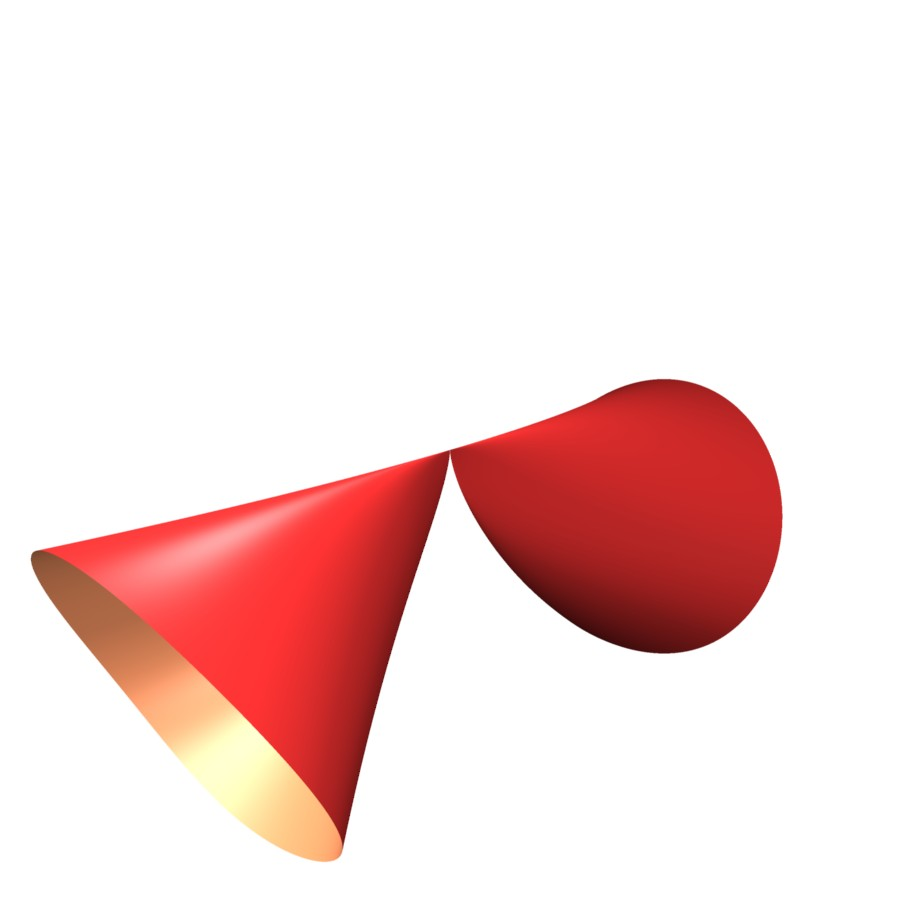
\includegraphics[width=1.1cm]{../../common/images/D5mm_01}
        \end{tabular}
      \end{tabular}
    \end{center}
    \vspace*{-0.4em}

We can also, as in the $D_5^{+-}$ case, make two $A_1$s and an $A_2$ singularity appear
when deforming in another way.

    \begin{center}
      \begin{tabular}{@{}c@{\quad}c@{\quad}c@{}}
        \begin{tabular}{@{}c@{}}
          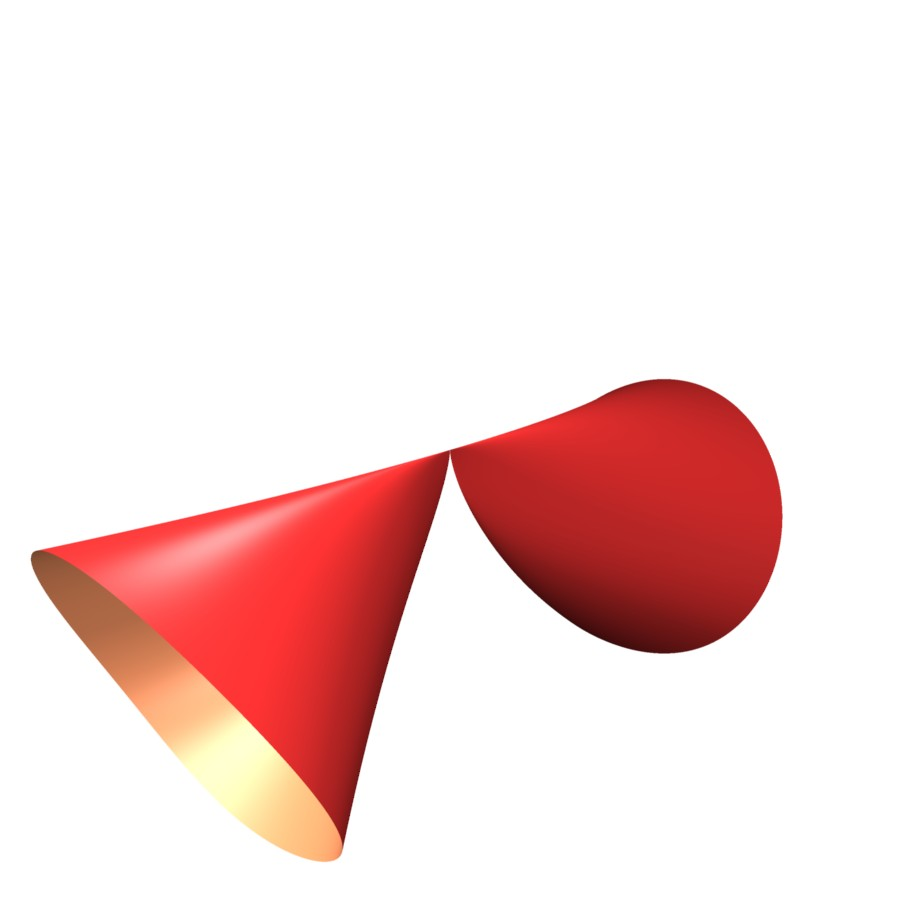
\includegraphics[width=1.1cm]{../../common/images/D5mm_01}
        \end{tabular}
        &
        \begin{tabular}{@{}c@{}}
          
\includegraphics[width=1.1cm]{../../common/images/D5mm_04}
        \end{tabular}
        &
        \begin{tabular}{@{}c@{}}
          
\includegraphics[width=1.1cm]{../../common/images/D5mm_05}
        \end{tabular}
      \end{tabular}
    \end{center}
    \vspace*{-0.4em}

\end{surferPage}
